\part{常见错误}
%Frequently Asked Questions
\section{boot分区剩余空间不足}
\begin{description}
\item[问题] \textcolor{red}{boot分区剩余空间不足}\\
\begin{figure}[!htbp]
	\centering
	\caption{boot分区剩余空间不足}  
		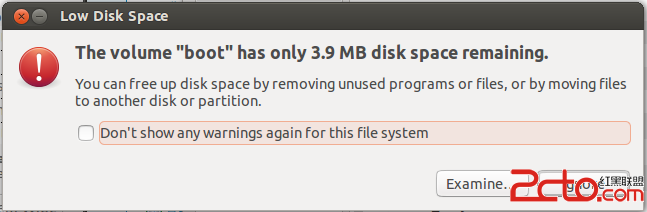
\includegraphics[scale=0.35]{figs/boot_space.png}
    	\label{fig:boot_space}
\end{figure}
\item[原因] \textcolor{blue}{
boot分区里面存放的是系统引导文件和内核的一些东西,这些东西100M是足够容纳的。而大家都知道linux内核一直在更新,跟新后,旧的内核就不在使用,但旧的内核文件还在boot里面,占据着空间,更新几次过后boot文件就会被占满,显示boot磁盘空间不足。这时为了更新需要将不用的内核文件删除,释放空间。
}
\item[方案]
\begin{enumerate}
\item 查看已安装的linux-image各版本\\
\begin{lstlisting}[style=BASH]
hjy@jy:~$ dpkg --get-selections | grep linux-image
\end{lstlisting}

\item 查看当前正在使用的镜像版本\\
\begin{lstlisting}[style=BASH]
hjy@jy:~$ uname -a
\end{lstlisting}

\item 卸载老版本\textcolor{red}{建议保留最新的两个版本}
\begin{lstlisting}[style=BASH]
hjy@jy:~$ sudo apt-get purge linux-image-3.x.x-xx-generic
\end{lstlisting}

\end{enumerate}

\end{description}
